\section{Реализация биржи}
\subsection{Общая архитектура}
Поговорим теперь о реализации биржевой инфраструктуры. Нашей целью будет написать главные компоненты биржи и обеспечить их совместную работу.
Рассмотрим внутреннюю архитектуру типичной биржи. В качестве примера возьмем одну из самых крупных и известных - Чикагская биржа \textbf{CME} [1.2]

\begin{center}
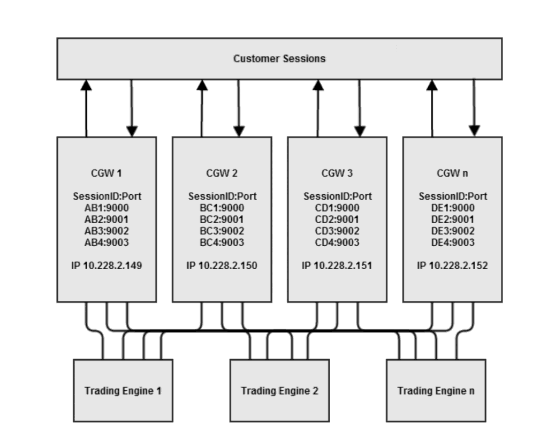
\includegraphics[width=400pt]{images/cme_schema.png}
\end{center}

Как можно видеть, главными компонентами биржи являются уже упомянутые выше торговые движки (Trading Engines в терминологии книги [1.2]). Посредником между ними и клиентами на этой схеме являются порты. Однако в реальности порты не только обеспечивают канал связи с клиентом, принимая его запросы (как это обычно принято подразумевать под термином "порт"), но и фильтруют их, предобрабатывают и распределяют очередь запросов, которую обрабатывает нужный торговый движок. Таким образом, более широкое и применимое определение этой сущности - \textbf{Connection Manager}.

В рамках этой работы будет рассмотрена упрощенная схема с одним торговым движком:

\begin{center}
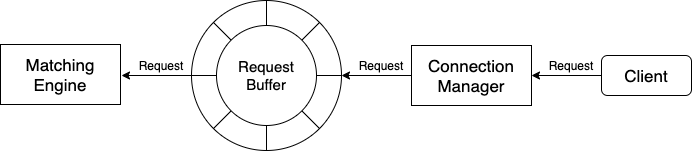
\includegraphics[width=400pt]{images/exchange_schema.png}
\end{center}


\textbf{Request Buffer} - это буффер запросов, куда они кладутся после поступления. Он будет асинхронно освобождаться торговым движком. Это один из ключевых компонентов с точки зрения нагрузоустойчивости: при его переполнении торги останавливаются до тех пор, пока все запросы не будут выполнены. Задача биржи устроить торги и инфраструктуру таким образом, чтобы этого не происходило.

\subsection{Backend}

Для написания бекенд части, я выбрал язык программирования \textbf{С++}. Он является низкоуровневым, высокопроизводительным и отказоустойчивым при правильной разработке. Кроме того, C++ в целом является стандартом разработки нагруженных компонент в финансовой индустрии.

Репозиторий с кодом открыт и находится по адресу

\begin{center} \url{https://github.com/evgenstf/market_load_prediction} \end{center}

При разработке я старался уделять большое внимания чистоте кода [3.1], правильным паттернам, тестам [3.2]  и общей логике[3.3].

Ниже представлена итоговая архитектура биржи, которая у меня получилась:


\begin{center}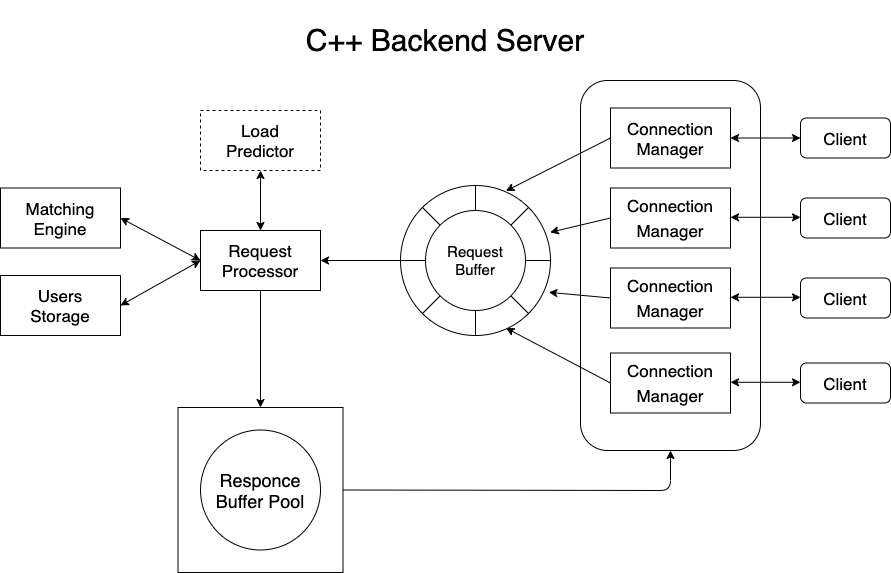
\includegraphics[width=450pt]{images/backend_schema.png}\end{center}

В ней присутствуют следующие основные компоненты:

\begin{itemize}
    \item \textbf{Connection Manager} - поддерживает соединение с клиентом по протоколу TCP и передает его запросы в \textbf{Request Buffer}.
    \item \textbf{Request Buffer} - асинхронное хранилище запросов.
    \item \textbf{Request Processor} - компонент, который достает запросы из \textbf{Request Buffer} и в зависимости от необходимой логики отправляет нужные команды в \textbf{Matching Engine} и. \textbf{User Storage}. После обработки запроса, отчет отправляется обратно в \textbf{Connection Manger} через \textbf{Response Pool}, который затем отправляется клиенту
    \item \textbf{User Storage} - сущность, хранящая личную информацию о клиентах: баланс, торговую историю, текущие заявки в биржевом стакане.
    \item \textbf{Matching Engine} - как уже было упомянуто, хранит биржевой стакан и обеспечивает логику сведения заявок в сделки.
    \item \textbf{Load Predictor} - компонент, предсказывающий нагрузку. О нем подробнее во второй части.
\end{itemize}


\newpage

\subsection{Frontend}

Для создания веб-интерфейса я использовал фреймворк под названием Django [3.4]. Это простое общеиспользуемое решение, которое легко применимо в данном случае.

Внутри содержится система изолированных каналов на основе Redis Server [3.5]. Это необходимо для того, чтобы поддерживать уникальное соединение с каждым пользователем по Websocket [3.6] (например, для отправки отчетов о сделках клиента) и отправлять пачку сообщений на группу пользователей, объединенных одним каналом (например, обновления стакана).

Фронтенд и бекенд серверы находятся на одной физической машине под управлением Ubuntu Server и общаются друг с другом посредством протокола TCP.

\begin{center}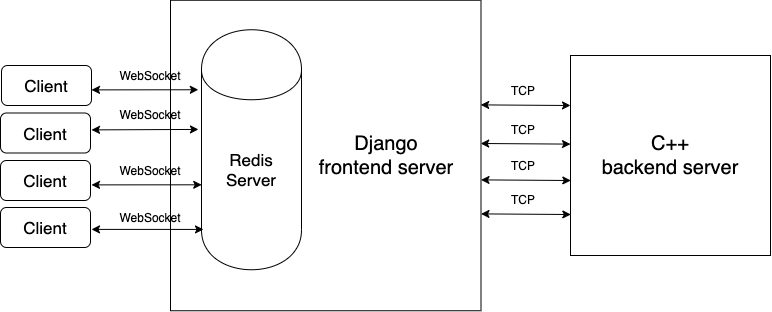
\includegraphics[width=450pt]{images/frontend_schema.png}\end{center}

\newpage
Веб интерфейс получился довольно лаконичным, и, в то же время, функциональным:

\begin{center}
    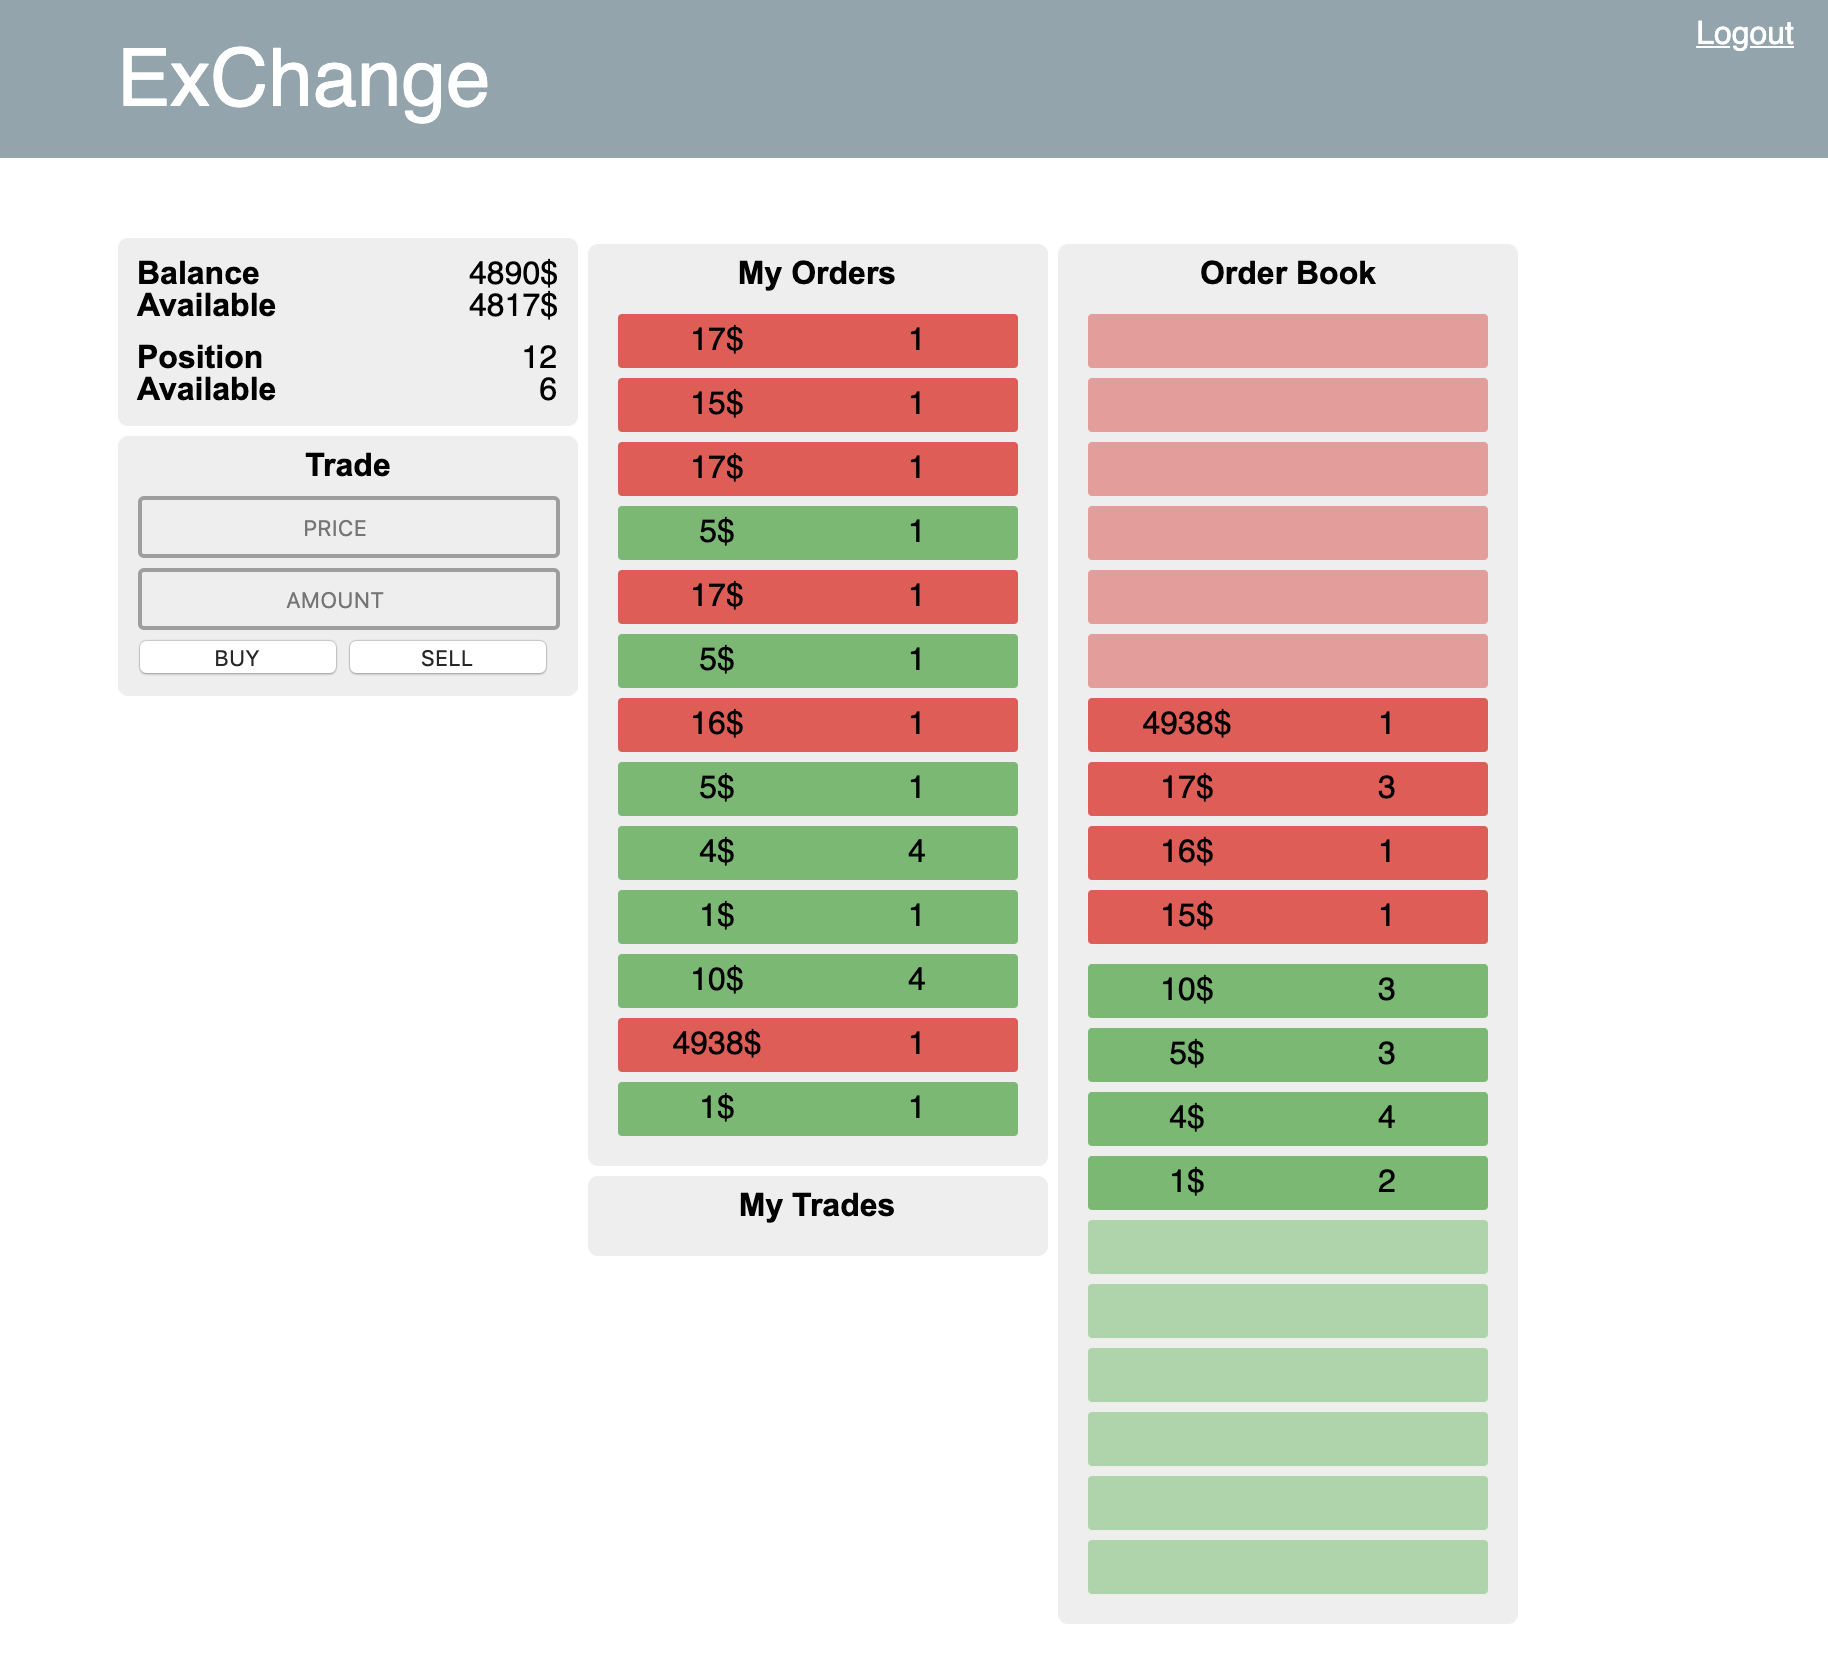
\includegraphics[width=450pt]{images/interface_screenshot.png}
\end{center}

Как можно видеть, на нем присутствуют: секция для отправки заявки, сделки пользователя, заявки пользователя, стоящие в стакане и, собственно, сам биржевой стакан.

\newpage
\subsection{Нагрузочное тестирование }

Для нагрузочного тестирования и проверки предсказывающих моделей был разработан CLI (Command line interface) инструмент, который эмулирует участника торгов и посылает заявки с конфигурируемым разбросом цен, объемом и частотой.

Я запустил его с несколькими значениями частоты отправки запросов и засек время, через которое буффер запросов переполняется. В таблице ниже представлены эти значения:


\begin{center}
\begin{tabular}{ c c }
 Requests per sec & Time till overflow in sec \\ 
 <1000 & $+\infty$\\
 1500-2500 & 950 \\
 2500-3500 & 300 \\
 3500-10000 & 100 \\
\end{tabular}
\end{center}

Отсюда можно сказать, что опытным путем была установлена производительность написанной биржи: 1000-1500 запросов в секунду (один запрос занимает от 600 до 1000 микросекунд).


\newpage
